\documentclass{article}
\usepackage{graphicx}
\graphicspath{ {images/} }
\usepackage{scrextend}
\usepackage[utf8]{inputenc}
\usepackage{color}   %May be necessary if you want to color links
\usepackage{hyperref}
\hypersetup{
    colorlinks=false, %set true if you want colored links
    linktoc=all,     %set to all if you want both sections and subsections linked
    linkcolor=blue,  %choose some color if you want links to stand out
}

\title{COP290: Institute Level Complaint Management
System}
\author{Aayan Kumar (2014CS10201) \\ Shreyan Gupta (2014CS10485) \\ Vaibhav Bhagee (2014CS50297) }
\date{10 March, 2016}

\begin{document}

\maketitle
 
\tableofcontents
\newpage
\section{Introduction}
    \par
    In this assignment we try to implement a basic Complaint Management System for IIT Delhi.  
    The app will cater to people of the institute like faculties, students and institute employee. 
    \par 
    Users with any grievances can submit their complaint and alert the concerned authorities.  A complaint is visible to all people who are affected by it, and all such users can express their views on a particular complaint in the form of threads and comments.
    \par
    The concerned authorities would take appropriate steps to resolve the complaint, and mark them as under resolution. If the end users are satisfied with the action of the authorities then the complaint would be marked as resolved, otherwise it would be forwarded to a higher authority.

\section{Scope of Assignment}
    \begin{addmargin}[1em]{2em}
    \subsection{Current Aim}
        Currently we are focusing on making an Android App which does the basic functionality of lodging a new complaint (for students) and viewing unresolved complaints.
    \end{addmargin}
    \begin{addmargin}[1em]{2em}
    \subsection{Possible future improvements}
        \par
        We can easily extend the app to cater to complaints by faculty and staff as well. 
        \par
        The assignment can be further extended to iOS, Windows as well as web apps in addition to android clients. 
    \end{addmargin}
    
\section{Implementation Details}
    \begin{addmargin}[1em]{2em}
    \subsection{Types of Complaints}
        There are 2 types of complaints we would be implementing
        \begin{itemize}
            \item The \textbf{Individual Complaints} are complaints which are posted by the user and the complaint directly goes to the concerned authority
            \item The \textbf{Community Complaints} are complaints which when posted by any user are visible to all concerned users defined by certain \textbf{Tags}. These include hostel level complaints and institute level complaints
        \end{itemize}
    \end{addmargin}    
    \begin{addmargin}[1em]{2em}
    \subsection{Field of Complaints}
        The complaints can be broadly divided into the following
        \begin{itemize}
            \item \textbf{Maintenance}: Ex. Broken door in hostel or geyser not working.
            \item \textbf{Mess}: Ex. Mess food not upto the mark
            \item \textbf{Student Welfare Related Complaint} 
            \item \textbf{Infrastructure}: Ex. Bad quality of seats in lecture halls.
            \item \textbf{Course related}: Complaints specific to courses.
            \item \textbf{NSO/ NSS/ NCC}
            \item \textbf{Security Complaint}: Ex: Stolen laptop, Ragging
        \end{itemize}
    \end{addmargin}

\section{Database Structure}

The database we are implementing is in MongoDB. It is a NoSQL type database and all the objects would be stored as a collection of JSON Objects. The Collection of objects along with their description is described below.


% Collection
    \begin{table}[ht]
    \centering
    \caption{Database Collections}
    \label{my-label}
    \begin{tabular}{|c|l|c|}
    \hline
    \multicolumn{3}{|c|}{\textbf{Database: Complaint Management System}}                                                                                    \\ \hline
    \multicolumn{2}{|c|}{\textbf{Collections}} & \textbf{Description}                                                                                       \\ \hline
    \multicolumn{2}{|c|}{Users}                & \begin{tabular}[c]{@{}c@{}}Collection of all the\\ users registered in the system\end{tabular}             \\ \hline
    \multicolumn{2}{|c|}{Special\_Users}       & \begin{tabular}[c]{@{}c@{}}Collection of all the special \\ users in the system\end{tabular}               \\ \hline
    \multicolumn{2}{|c|}{Complaints}           & \begin{tabular}[c]{@{}c@{}}Collection of all the complaints\\ (Both individual and community)\end{tabular} \\ \hline
    \multicolumn{2}{|l|}{Notifications}        & \multicolumn{1}{l|}{Collection of all the notifications}                                                   \\ \hline
    \end{tabular}
    \end{table}







\begin{itemize}
    \newpage
    \item The User and Special User Collections are made up of User JSON Objects.
    \begin{itemize}
    	\item The User Object corresponds to each individual user of the Complaint System. This includes Students, Professors and Faculty Members. The structure of the User object is described in the table below.
	    \end{itemize}
    	% JSON object for User    
        \begin{table}[ht]
        \centering
        \caption{User JSON Object}
        \label{my-label}
        \begin{tabular}{|c|c|c|}
        \hline
        \textbf{Field\_Names} & \textbf{Type} & \textbf{Description} \\ \hline
        Unique ID & String & \begin{tabular}[c]{@{}c@{}}PRIMARY KEY\\ This is the unique identification number of\\ i.e Entry Number for the students and registration\\ id for faculty and staff\end{tabular} \\ \hline
        Name & String & Name of the User \\ \hline
        Password & String & Hashed password of the User \\ \hline
        Department & String & Associated Department \\ \hline
        \begin{tabular}[c]{@{}c@{}}Contact\\ Information\end{tabular} & String & Contact information of the user \\ \hline
        Tags & \begin{tabular}[c]{@{}c@{}}String \\ Array\end{tabular} & \begin{tabular}[c]{@{}c@{}}A list of the tags to which a user is associated\\ (eg. Hostel, NCC/NSS/NSO etc)\end{tabular} \\ \hline
        Complaint List & \begin{tabular}[c]{@{}c@{}}String \\ Array\end{tabular} & \begin{tabular}[c]{@{}c@{}}An array of complaint IDs of the complaints to \\ which a user is associated\end{tabular} \\ \hline
        Courses List & \begin{tabular}[c]{@{}c@{}}String\\ Array\end{tabular} & A list of courses in which the user in enrolled \\ \hline
        \end{tabular}
        \end{table}
        \newpage

    \item The Complaints Collections are made up of Individual Complaint Objects and Community Complaint Objects.
    \begin{itemize}
    	\item The Individual Complaint Object corresponds to a complaint which would only be visible to the lodger of the complaint and the concerned authority.
        % JSON object for individual complaints
        \begin{table}[ht]
        \centering
        \caption{Individual Complaint JSON Object}
        \label{my-label}
        \begin{tabular}{|c|c|c|}
        \hline
        \multicolumn{3}{|c|}{\textbf{Individual Complaint JSON Object description}} \\ \hline
        \textbf{Field\_Names} & \textbf{Type} & \textbf{Description} \\ \hline
        Complaint ID & String & \begin{tabular}[c]{@{}c@{}}PRIMARY KEY\\ This is the unique identification number of\\ the complaint\end{tabular} \\ \hline
        Lodged\_By & String & \begin{tabular}[c]{@{}c@{}}FOREIGN KEY\\ Unique ID of the User who lodged \\ the complaint\end{tabular} \\ \hline
        Title & String & Title of the complaint \\ \hline
        Description & String & Description of the complaint \\ \hline
        Timestamp & \begin{tabular}[c]{@{}c@{}}Timestamp\\ JSON\\ Object\end{tabular} & \begin{tabular}[c]{@{}c@{}}A JSON object to store the \\                  a. Date of Lodging of complaint\\ b. Date of last update\end{tabular} \\ \hline
        Is\_Community & Boolean & \begin{tabular}[c]{@{}c@{}}A flag to store whether the complaint is \\ individual type or not\end{tabular} \\ \hline
        Type & String & \begin{tabular}[c]{@{}c@{}}The broad area, from the Hierarchy Tree \\ to which the complaint is related\end{tabular} \\ \hline
        \begin{tabular}[c]{@{}c@{}}Authority\\ Hierarchy\end{tabular} & \begin{tabular}[c]{@{}c@{}}JSON\\ Object\end{tabular} & \begin{tabular}[c]{@{}c@{}}A JSON object which stores the hierarchy\\ of the complaint type\end{tabular} \\ \hline
        Current\_Level & String & \begin{tabular}[c]{@{}c@{}}The current authority level with \\ whom the complaint resides\end{tabular} \\ \hline
        Current\_Status & String & \begin{tabular}[c]{@{}c@{}}Either one of below values\\ Unresolved/Resolved/Under\_Resolution\end{tabular} \\ \hline
        \begin{tabular}[c]{@{}c@{}}Associated\\ Threads\end{tabular} & \begin{tabular}[c]{@{}c@{}}Threads\\ Object\\ Array\end{tabular} & \begin{tabular}[c]{@{}c@{}}The list of threads related to the\\ current complaint\end{tabular} \\ \hline
        \end{tabular}
        \end{table}
        \newpage
    
    	\item The Community Complaint Object corresponds to a complaint which would be visible to the lodger of the complaint, the concerned authority, along with all the people who share the tag which corresponds to the complaint.
        % JSON object for community complaint
        \begin{table}[ht]
        \centering
        \caption{Community Complaint JSON Object}
        \label{my-label}
        \begin{tabular}{|c|c|c|}
        \hline
        \multicolumn{3}{|c|}{\textbf{Community Complaint JSON Object description}} \\ \hline
        \textbf{Field\_Names} & \textbf{Type} & \textbf{Description} \\ \hline
        Complaint ID & String & \begin{tabular}[c]{@{}c@{}}PRIMARY KEY\\ This is the unique identification number of\\ the complaint\end{tabular} \\ \hline
        Lodged\_By & String & \begin{tabular}[c]{@{}c@{}}FOREIGN KEY\\ Unique ID of the User who lodged \\ the complaint\end{tabular} \\ \hline
        Title & String & Title of the complaint \\ \hline
        Description & String & Description of the complaint \\ \hline
        Timestamp & \begin{tabular}[c]{@{}c@{}}Timestamp\\ JSON\\ Object\end{tabular} & \begin{tabular}[c]{@{}c@{}}A JSON object to store the \\                  a. Date of Lodging of complaint\\ b. Date of last update\end{tabular} \\ \hline
        Is\_Community & Boolean & \begin{tabular}[c]{@{}c@{}}A flag to store whether the complaint is \\ individual type or not\end{tabular} \\ \hline
        Type & String & \begin{tabular}[c]{@{}c@{}}The broad area, from the Hierarchy Tree \\ to which the complaint is related\end{tabular} \\ \hline
        \begin{tabular}[c]{@{}c@{}}Authority\\ Hierarchy\end{tabular} & \begin{tabular}[c]{@{}c@{}}JSON\\ Object\end{tabular} & \begin{tabular}[c]{@{}c@{}}A JSON object which stores the hierarchy\\ of the complaint type\end{tabular} \\ \hline
        Current\_Level & String & \begin{tabular}[c]{@{}c@{}}The current authority level with \\ whom the complaint resides\end{tabular} \\ \hline
        Current\_Status & String & \begin{tabular}[c]{@{}c@{}}Either one of below values\\ Unresolved/Resolved/Under\_Resolution\end{tabular} \\ \hline
        Votes & Vote Object & \begin{tabular}[c]{@{}c@{}}A vote object which stores the information\\ of number of up-votes, down-votes and list of\\ people who have voted\end{tabular} \\ \hline
        \begin{tabular}[c]{@{}c@{}}Associated\\ Threads\end{tabular} & \begin{tabular}[c]{@{}c@{}}Threads\\ Object\\ Array\end{tabular} & \begin{tabular}[c]{@{}c@{}}The list of threads related to the\\ current complaint\end{tabular} \\ \hline
        \end{tabular}
        \end{table}
    	\newpage
    	
    	\item The Vote JSON Object corresponds to the vote associated with a single Community Complaint.
        % JSON object of vote
        \begin{table}[ht]
        \centering
        \caption{Vote JSON Object}
        \label{my-label}
        \begin{tabular}{|c|c|c|}
        \hline
        \multicolumn{3}{|c|}{\textbf{Vote JSON Object description}} \\ \hline
        \textbf{Field\_Names} & \textbf{Type} & \textbf{Description} \\ \hline
        \begin{tabular}[c]{@{}c@{}}No. of\\ Upvotes\end{tabular} & Integer & Number of upvotes \\ \hline
        \begin{tabular}[c]{@{}c@{}}No. of\\ Downvotes\end{tabular} & Integer & Number of Downvotes \\ \hline
        \begin{tabular}[c]{@{}c@{}}People\\ Voted\end{tabular} & String Array & \begin{tabular}[c]{@{}c@{}}Array of Unique ID of\\ people who have voted\end{tabular} \\ \hline
        \end{tabular}
        \end{table}
        

    	\item The Thread Object corresponds to a single thread that would be associated with a single Community Complaint.
        % JSON object of thread
        \begin{table}[ht]
        \centering
        \caption{Thread JSON Object}
        \label{my-label}
        \begin{tabular}{|c|c|c|}
        \hline
        \multicolumn{3}{|c|}{\textbf{Thread JSON Object description}} \\ \hline
        \textbf{Field\_Names} & \textbf{Type} & \textbf{Description} \\ \hline
        Thread\_ID & String & \begin{tabular}[c]{@{}c@{}}PRIMARY KEY\\ This is the unique identification number of\\ the thread\end{tabular} \\ \hline
        Complaint\_ID & String & \begin{tabular}[c]{@{}c@{}}FOREIGN KEY\\ Unique ID of the Complaint to\\ which the thread is associated\end{tabular} \\ \hline
        Title & String & Title of the thread \\ \hline
        Description & String & Description of the thread \\ \hline
        \begin{tabular}[c]{@{}c@{}}Last\\ Updated\end{tabular} & Timestamp & Date of last update \\ \hline
        \begin{tabular}[c]{@{}c@{}}Associated\\ Comments\end{tabular} & \begin{tabular}[c]{@{}c@{}}Comments\\ Object\\ Array\end{tabular} & \begin{tabular}[c]{@{}c@{}}The list of comments related to the\\ current thread\end{tabular} \\ \hline
        \end{tabular}
        \end{table}
        \newpage

    	\item The Comment Object corresponds to a single comment what would be associated with a single Thread.
       	% JSON object of comment
        \begin{table}[ht]
        \centering
        \caption{Comment JSON Object}
        \label{my-label}
        \begin{tabular}{|c|c|c|}
        \hline
        \multicolumn{3}{|c|}{\textbf{Comment JSON Object description}} \\ \hline
        \textbf{Field\_Names} & \textbf{Type} & \textbf{Description} \\ \hline
        Posted\_By & String & \begin{tabular}[c]{@{}c@{}}This is the unique identification number of\\ the person who posted the comment\end{tabular} \\ \hline
        Description & String & Description of the thread \\ \hline
        Posted On & Timestamp & Date and time of Posting Comment \\ \hline
        \end{tabular}
        \end{table}
    \end{itemize}

    \item The Notification Collection is made up of Notification JSON Objects
     \begin{itemize}
    	\item The Notification JSON Object has the information of a specific notification generated on updation of a complaint, along with the time stamp.
    \end{itemize}
    
    
\end{itemize}


    
%Notification JSON    
    \begin{table}[ht]
    \centering
    \caption{Notification JSON Object}
    \label{my-label}
    \begin{tabular}{|c|c|c|}
    \hline
    \multicolumn{3}{|c|}{\textbf{Notification JSON object description}}                                                                        \\ \hline
    \textbf{Field} & \textbf{Type} & \textbf{Description}                                                                                      \\ \hline
    Complaint ID   & String        & \begin{tabular}[c]{@{}c@{}}Unique ID of the complaint to\\ which the notification is related\end{tabular} \\ \hline
    Timestamp      & String        & Time of the notification                                                                                  \\ \hline
    Content        & String        & \begin{tabular}[c]{@{}c@{}}The content to be displayed\\ in the notification\end{tabular}                 \\ \hline
    \end{tabular}
    \end{table}
    
%Time Person Place
%Timestamp JSON
    \begin{table}[ht]
    \centering
    \caption{Timestamp JSON Object}
    \label{my-label}
    \begin{tabular}{|c|c|c|}
    \hline
    \multicolumn{3}{|c|}{\textbf{Timestamp JSON object description}}                                                      \\ \hline
    \textbf{Field}  & \textbf{Type} & \textbf{Description}                                                                \\ \hline
    Time of Lodging & String        & \begin{tabular}[c]{@{}c@{}}Timestamp of lodging\\ the complaint\end{tabular}        \\ \hline
    Last Update     & String        & \begin{tabular}[c]{@{}c@{}}Timestamp of last\\ update of the complaint\end{tabular} \\ \hline
    \end{tabular}
    \end{table}

%Hierarchy JSON object
    \begin{table}[ht]
    \centering
    \caption{Hierarchy JSON Object}
    \label{my-label}
    \begin{tabular}{|c|c|c|}
    \hline
    \multicolumn{3}{|c|}{\textbf{Hierarchy JSON object description}} \\ \hline
    \textbf{Field} & \textbf{Type} & \textbf{Description} \\ \hline
    Hostel Lists & \begin{tabular}[c]{@{}c@{}}JSON\\ Array of\\ Hostel Objects\end{tabular} & \begin{tabular}[c]{@{}c@{}}Array of Hostel JSON \\ Objects\end{tabular} \\ \hline
    \begin{tabular}[c]{@{}c@{}}Student\\ Welfare\\ Complaint\end{tabular} & \begin{tabular}[c]{@{}c@{}}Student\\ Welfare Complaint\\ Object\end{tabular} & \begin{tabular}[c]{@{}c@{}}Contains Hierarchy of \\ Student Welfare\\ Complaints\end{tabular} \\ \hline
    \begin{tabular}[c]{@{}c@{}}Infrastructure\\ Complaint\end{tabular} & \begin{tabular}[c]{@{}c@{}}Infrastructure Complaint\\ Object\end{tabular} & \begin{tabular}[c]{@{}c@{}}Contains Hierarchy of\\ Infrastuctue Complaints\end{tabular} \\ \hline
    Course Complaint & Course Complaint Object & \begin{tabular}[c]{@{}c@{}}Contains Hierarchy of \\ course complaints\end{tabular} \\ \hline
    \begin{tabular}[c]{@{}c@{}}NCC/NSO/NSS\\ Complaint\end{tabular} & N\_Complaint\_Object & \begin{tabular}[c]{@{}c@{}}Contains Hierarchy of\\ NCC/NSS/NSO complaints\end{tabular} \\ \hline
    Security Complaint & Security Complaint Object & \begin{tabular}[c]{@{}c@{}}Contains Hierarchy of \\ Security Complaints\end{tabular} \\ \hline
    \end{tabular}
    \end{table}
    
    
    \begin{figure}[h]
            \centering
            \includegraphics[width=1.0\textwidth,height=0.6\textwidth]{Complaint_Hierarchy}
            \caption{Complaint Hierarchy}
            \label{fig:my_label}
        \end{figure}
    
% %Hostel JSON Object
%     \begin{table}[ht]
%     \centering
%     \caption{Hostel JSON Object}
%     \label{my-label}
%     \begin{tabular}{|c|c|c|}
%     \hline
%     \multicolumn{3}{|c|}{\textbf{Hostel JSON object description}} \\ \hline
%     \textbf{Field} & \textbf{Type} & \textbf{Description} \\ \hline
%     Name & String & Name of Hostel \\ \hline
%     \begin{tabular}[c]{@{}c@{}}Mess\\ Complaint\end{tabular} & \begin{tabular}[c]{@{}c@{}}Mess Complaint\\ Object\end{tabular} & \begin{tabular}[c]{@{}c@{}}Contains Hierarchy of \\ Mess\\ Complaints\end{tabular} \\ \hline
%     \begin{tabular}[c]{@{}c@{}}Maintenance\\ Complaint\end{tabular} & \begin{tabular}[c]{@{}c@{}}Maintenance Complaint\\ Object\end{tabular} & \begin{tabular}[c]{@{}c@{}}Contains Hierarchy of\\ Maintenance Complaints\end{tabular} \\ \hline
%     \end{tabular}
%     \end{table}
    
% %Mess Complaint JSON Object
%     \begin{table}[ht]
%     \centering
%     \caption{Mess Complaint JSON Object}
%     \label{my-label}
%     \begin{tabular}{|l|l|l|}
%     \hline
%     \multicolumn{3}{|l|}{\textbf{Mess Complaint Object Description}}                                                                                                     \\ \hline
%     \textbf{Field}                                                      & \textbf{Type} & \textbf{Description}                                                           \\ \hline
%     \begin{tabular}[c]{@{}l@{}}Mess\\ Secretary\end{tabular}            & String        & \begin{tabular}[c]{@{}l@{}}Unique ID of\\ Mess Secretary\end{tabular}          \\ \hline
%     \begin{tabular}[c]{@{}l@{}}House\\ Secretary\end{tabular}           & String        & \begin{tabular}[c]{@{}l@{}}Unique ID of \\ House Secretary\end{tabular}        \\ \hline
%     Warden                                                              & String        & \begin{tabular}[c]{@{}l@{}}Unique ID of \\ Warden\end{tabular}                 \\ \hline
%     \begin{tabular}[c]{@{}l@{}}Associate\\ Dean, HM\end{tabular}        & String        & \begin{tabular}[c]{@{}l@{}}Unique ID of\\ Associate Dean, HM\end{tabular}      \\ \hline
%     \begin{tabular}[c]{@{}l@{}}Dean, \\ Student \\ Affairs\end{tabular} & String        & \begin{tabular}[c]{@{}l@{}}Unique ID of\\ Dean, Student\\ Affairs\end{tabular} \\ \hline
%     Director                                                            & String        & \begin{tabular}[c]{@{}l@{}}Unique ID of\\ Director\end{tabular}                \\ \hline
%     \end{tabular}
%     \end{table}
    
% %Maintenance Complaint JSON Object
%     \begin{table}[ht]
%     \centering
%     \caption{Maintenance Complaint JSON Object}
%     \label{my-label}
%     \begin{tabular}{|l|l|l|}
%     \hline
%     \multicolumn{3}{|l|}{\textbf{Maintenance Complaint Object Description}}                                                                                                     \\ \hline
%     \textbf{Field}                                                      & \textbf{Type} & \textbf{Description}                                                           \\ \hline
%     \begin{tabular}[c]{@{}l@{}}Maintenance\\ Secretary\end{tabular}            & String        & \begin{tabular}[c]{@{}l@{}}Unique ID of\\ Maintenance Secretary\end{tabular}          \\ \hline
%     \begin{tabular}[c]{@{}l@{}}House\\ Secretary\end{tabular}           & String        & \begin{tabular}[c]{@{}l@{}}Unique ID of \\ House Secretary\end{tabular}        \\ \hline
%     Warden                                                              & String        & \begin{tabular}[c]{@{}l@{}}Unique ID of \\ Warden\end{tabular}                 \\ \hline
%     \begin{tabular}[c]{@{}l@{}}Associate\\ Dean, HM\end{tabular}        & String        & \begin{tabular}[c]{@{}l@{}}Unique ID of\\ Associate Dean, HM\end{tabular}      \\ \hline
%     \begin{tabular}[c]{@{}l@{}}Dean, \\ Student \\ Affairs\end{tabular} & String        & \begin{tabular}[c]{@{}l@{}}Unique ID of\\ Dean, Student\\ Affairs\end{tabular} \\ \hline
%     Director                                                            & String        & \begin{tabular}[c]{@{}l@{}}Unique ID of\\ Director\end{tabular}                \\ \hline
%     \end{tabular}
%     \end{table}    
    
% %Student Welfare Complaint Object
%     \begin{table}[ht]
%     \centering
%     \caption{Student Welfare Complaint Object}
%     \label{my-label}
%     \begin{tabular}{|l|l|l|}
%     \hline
%     \multicolumn{3}{|l|}{\textbf{Student Welfare Complaint Object Description}} \\ \hline
%     \textbf{Field} & \textbf{Type} & \textbf{Description} \\ \hline
%     \begin{tabular}[c]{@{}l@{}}BSW \\ General\\ Secretary\end{tabular} & String & \begin{tabular}[c]{@{}l@{}}Unique ID of\\ BSW General\\ Secretary\end{tabular} \\ \hline
%     \begin{tabular}[c]{@{}l@{}}SAC \\ General \\ Secretary\end{tabular} & String & \begin{tabular}[c]{@{}l@{}}Unique ID of \\ SAC General\\ Secretary\end{tabular} \\ \hline
%     \begin{tabular}[c]{@{}l@{}}President\\ SAC\end{tabular} & String & \begin{tabular}[c]{@{}l@{}}Unique ID of\\ President SAC\end{tabular} \\ \hline
%     \begin{tabular}[c]{@{}l@{}}Dean, \\ Student \\ Affairs\end{tabular} & String & \begin{tabular}[c]{@{}l@{}}Unique ID of\\ Dean, Student\\ Affairs\end{tabular} \\ \hline
%     Director & String & \begin{tabular}[c]{@{}l@{}}Unique ID of\\ Director\end{tabular} \\ \hline
%     \end{tabular}
%     \end{table}
    
% %Infrastructure Complaint Object
%     \begin{table}[ht]
%     \centering
%     \caption{Infrastructure Complaint Object}
%     \label{my-label}
%     \begin{tabular}{|l|l|l|}
%     \hline
%     \multicolumn{3}{|l|}{\textbf{Infrastructure Complaint Object Description}} \\ \hline
%     \textbf{Field} & \textbf{Type} & \textbf{Description} \\ \hline
%     \begin{tabular}[c]{@{}l@{}}BHM \\ General\\ Secretary\end{tabular} & String & \begin{tabular}[c]{@{}l@{}}Unique ID of\\ BHM General\\ Secretary\end{tabular} \\ \hline
%     \begin{tabular}[c]{@{}l@{}}SAC \\ General \\ Secretary\end{tabular} & String & \begin{tabular}[c]{@{}l@{}}Unique ID of \\ SAC General\\ Secretary\end{tabular} \\ \hline
%     \begin{tabular}[c]{@{}l@{}}President\\ SAC\end{tabular} & String & \begin{tabular}[c]{@{}l@{}}Unique ID of\\ President SAC\end{tabular} \\ \hline
%     \begin{tabular}[c]{@{}l@{}}Dean, \\ Student \\ Affairs\end{tabular} & String & \begin{tabular}[c]{@{}l@{}}Unique ID of\\ Dean, Student\\ Affairs\end{tabular} \\ \hline
%     Director & String & \begin{tabular}[c]{@{}l@{}}Unique ID of\\ Director\end{tabular} \\ \hline
%     \end{tabular}
%     \end{table}

% %Course Complaint Object
%     \begin{table}[ht]
%     \centering
%     \caption{Course Complaint Object}
%     \label{my-label}
%     \begin{tabular}{|l|l|l|}
%     \hline
%     \textbf{Field} & \textbf{Type} & \textbf{Description} \\ \hline
%     \begin{tabular}[c]{@{}l@{}}Course\\ Coordinator\end{tabular} & String & \begin{tabular}[c]{@{}l@{}}Unique ID of\\ Course Coordinator\end{tabular} \\ \hline
%     HOD & String & \begin{tabular}[c]{@{}l@{}}Unique ID of\\ HOD\end{tabular} \\ \hline
%     \begin{tabular}[c]{@{}l@{}}Dean,\\ Academics\end{tabular} & String & \begin{tabular}[c]{@{}l@{}}Unique ID of\\ Dean, Academics\end{tabular} \\ \hline
%     Director & String & \begin{tabular}[c]{@{}l@{}}Unique ID of\\ Director\end{tabular} \\ \hline
%     \end{tabular}
%     \end{table}

% %N_Complaint Object
%     \begin{table}[ht]
%     \centering
%     \caption{N_Complaint Object}
%     \label{my-label}
%     \begin{tabular}{|l|l|l|}
%     \hline
%     \textbf{Field} & \textbf{Type} & \textbf{Description} \\ \hline
%     \begin{tabular}[c]{@{}l@{}General \\ Secretary\end{tabular} & String & \begin{tabular}[c]{@{}l@{}}Unique ID of \\ General Secretary\end{tabular} \\ \hline
%     President, \\ NCC/NSS/NSO & String & \begin{tabular}[c]{@{}l@{}}Unique ID of \\ President \\ HOD\end{tabular} \\ \hline
%     \begin{tabular}[c]{@{}l@{}}Dean,\\ Academics\end{tabular} & String & \begin{tabular}[c]{@{}l@{}}Unique ID of\\ Dean, Academics\end{tabular} \\ \hline
%     Director & String & \begin{tabular}[c]{@{}l@{}}Unique ID of\\ Director\end{tabular} \\ \hline
%     \end{tabular}
%     \end{table}


%%%%%%%%%%%%%%%%%%%%%%%%%%%%%%%%%%%%%%%%%%%%%%    

\newpage
\clearpage
\section{APIs}
        \begin{figure}[h]
            \centering
            \includegraphics[width=1.0\textwidth,height=0.5\textwidth]{Login_API}
            \caption{Login API}
            \label{fig:my_label}
        \end{figure}
        \begin{figure}[h]
            \centering
            \includegraphics[width=1.0\textwidth,height=0.5\textwidth]{Login_special_API}
            \caption{Special Login API}
            \label{fig:my_label}
        \end{figure}
        \begin{figure}[h]
            \centering
            \includegraphics[width=1.0\textwidth,height=0.5\textwidth]{Add_user_API}
            \caption{Add User API}
            \label{fig:my_label}
        \end{figure}
        \begin{figure}[h]
            \centering
            \includegraphics[width=1.0\textwidth,height=0.5\textwidth]{Delete_USER_API}
            \caption{Delete User API}
            \label{fig:my_label}
        \end{figure}
        \begin{figure}[h]
            \centering
            \includegraphics[width=1.0\textwidth,height=0.5\textwidth]{Update_details_API}
            \caption{Update Details API}
            \label{fig:my_label}
        \end{figure}
        \begin{figure}[h]
            \centering
            \includegraphics[width=1.0\textwidth,height=0.5\textwidth]{List_of_complaints_API}
            \caption{List of Complaints API}
            \label{fig:my_label}
        \end{figure}
        \begin{figure}[h]
            \centering
            \includegraphics[width=1.0\textwidth,height=0.5\textwidth]{Complaint_details_API}
            \caption{Complaint Details API}
            \label{fig:my_label}
        \end{figure}
        \begin{figure}[h]
            \centering
            \includegraphics[width=1.0\textwidth,height=0.5\textwidth]{Get_notifications_API}
            \caption{Get Notifications API}
            \label{fig:my_label}
        \end{figure}
        \begin{figure}[h]
            \centering
            \includegraphics[width=1.0\textwidth,height=0.5\textwidth]{Add_complaint_API}
            \caption{Add Complaint API}
            \label{fig:my_label}
        \end{figure}
        \begin{figure}[h]
            \centering
            \includegraphics[width=1.0\textwidth,height=0.5\textwidth]{New_thread_API}
            \caption{New thread API}
            \label{fig:my_label}
        \end{figure}
        \begin{figure}[h]
            \centering
            \includegraphics[width=1.0\textwidth,height=0.5\textwidth]{New_Comment_API}
            \caption{New Comment API}
            \label{fig:my_label}
        \end{figure}
        \begin{figure}[h]
            \centering
            \includegraphics[width=1.0\textwidth,height=0.5\textwidth]{Mark_resolved_API}
            \caption{Mark Resolved API}
            \label{fig:my_label}
        \end{figure}
        \begin{figure}[h]
            \centering
            \includegraphics[width=1.0\textwidth,height=0.5\textwidth]{Relodge_higher_API}
            \caption{Relodge higher API}
            \label{fig:my_label}
        \end{figure}
        \begin{figure}[h]
            \centering
            \includegraphics[width=1.0\textwidth,height=0.5\textwidth]{Relodge_same_API}
            \caption{Relodge same API}
            \label{fig:my_label}
        \end{figure}
        \begin{figure}[h]
            \centering
            \includegraphics[width=1.0\textwidth,height=0.5\textwidth]{Vote_API}
            \caption{Vote API}
            \label{fig:my_label}
        \end{figure}
      
\clearpage
\section{Event Flow}
        \begin{figure}[h]
            \centering
            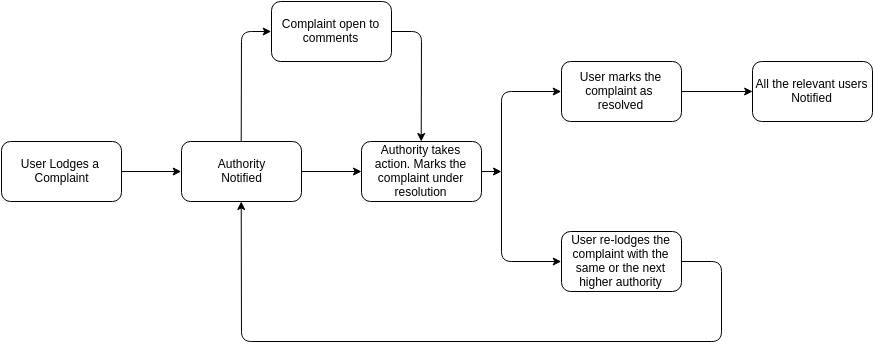
\includegraphics[width=1.0\textwidth,height=0.5\textwidth]{Individual_Complaint}
            \caption{Event flow for individual complaint}
            \label{fig:my_label}
        \end{figure}
        \begin{figure}[h]
            \centering
            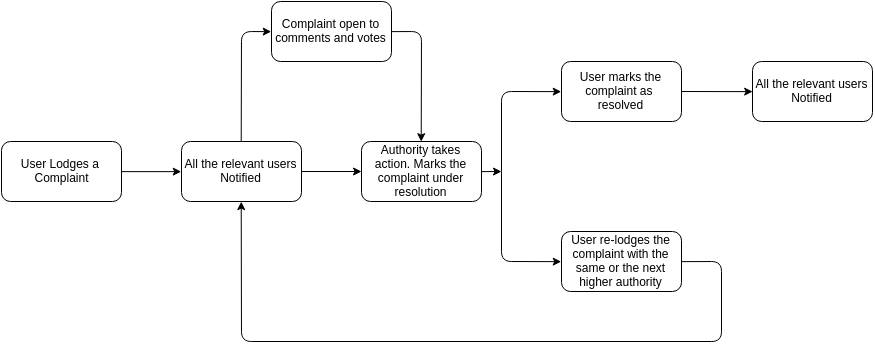
\includegraphics[width=1.0\textwidth,height=0.5\textwidth]{Community_Complaint}
            \caption{Event flow for community complaint}
            \label{fig:my_label}
        \end{figure}
        \clearpage
\section{User Interface}
    \begin{addmargin}[1em]{2em}

        \subsection{Login Page}
        The login page, as simple as it sounds, basically takes the user id and password input from the user and logs in the user
    \end{addmargin}
    \begin{addmargin}[1em]{2em}
            
        \subsection{Notification Page}
        Notification page would display a list of all recent notifications specific to the user. A notification is generated when a \textbf{new community complaint is posted}, or when a \textbf{new thread is added} to a complaint concerning the user or when a \textbf{new comment} is added to a thread
        
    \end{addmargin}
    \begin{addmargin}[1em]{2em}
        
        \subsection{Complaint Display Page}
        There are 3 types of complaint which would be displayed in 3 separate lists: Unresolved Complaints, Resolved Complaints and Complaints under Resolution.
        
    \end{addmargin}
    \begin{addmargin}[1em]{2em}
        
        \subsection{Complaint Lodging Page}
        This page takes details for a new complaint, like Title, Description, Field of Complaint, Type of Complaint and lodges it.
    \end{addmargin}
\section{References}
    \begin{itemize}
        \item https://www.draw.io/
        \item http://www.tablesgenerator.com/
        \item http://www.sharelatex.com/
    \end{itemize}

\end{document}